\chapter{System Model} 		\label{chp_sys_model}
One of main contribution of this paper is the analytical evaluation of the saturation analysis of 802.11ax OFDMA-based random access, in the assumption of ideal channel conditions (i.e., no hidden terminals and capture). 
The Markov chain model of random access was first proposed by Bianchi for analyzing distributed coordination function\cite{bianchi2000performance}. 
Here, for the brand new ODFMA-based random access, we generate a new Markov chain model. 
In this analysis, we generate three metrics, $n_s$ number of stations who succeed in contending in a stage, eff self-defined system efficiency, and $D$ access delay of request frame. 

The analysis is divided into two parts. First is the Markov chain model to estimate the packet transmission probability $\tau$ and conditional collision probability $p$. 
Secondly, we express the three metrics as function of $\tau$. 
Table \ref{table_notation} is a list of all parameters and notations.

Before generating Markov Chain model, we need to clarify concept of time in this mechanism.
The OFDMA-based random access is a three-way handshake procedure, AP initiating a TF, followed with STAs' sending request, then AP reponding the request with ACK.
The whole procedure is so-called "stage".
Actually, we have known that in legacy 802.11 DCF, time is measured in slot, which is a unit of time.
Here, time is measured in stage, which is a discrete time and is not synchronized with physical time. 
Stages should be mapped with "slot" in legacy random access mechanism.
Thus, access delay in this mechanism will be number of stages for station to access channel.

\begin{figure}[!t]
\centering
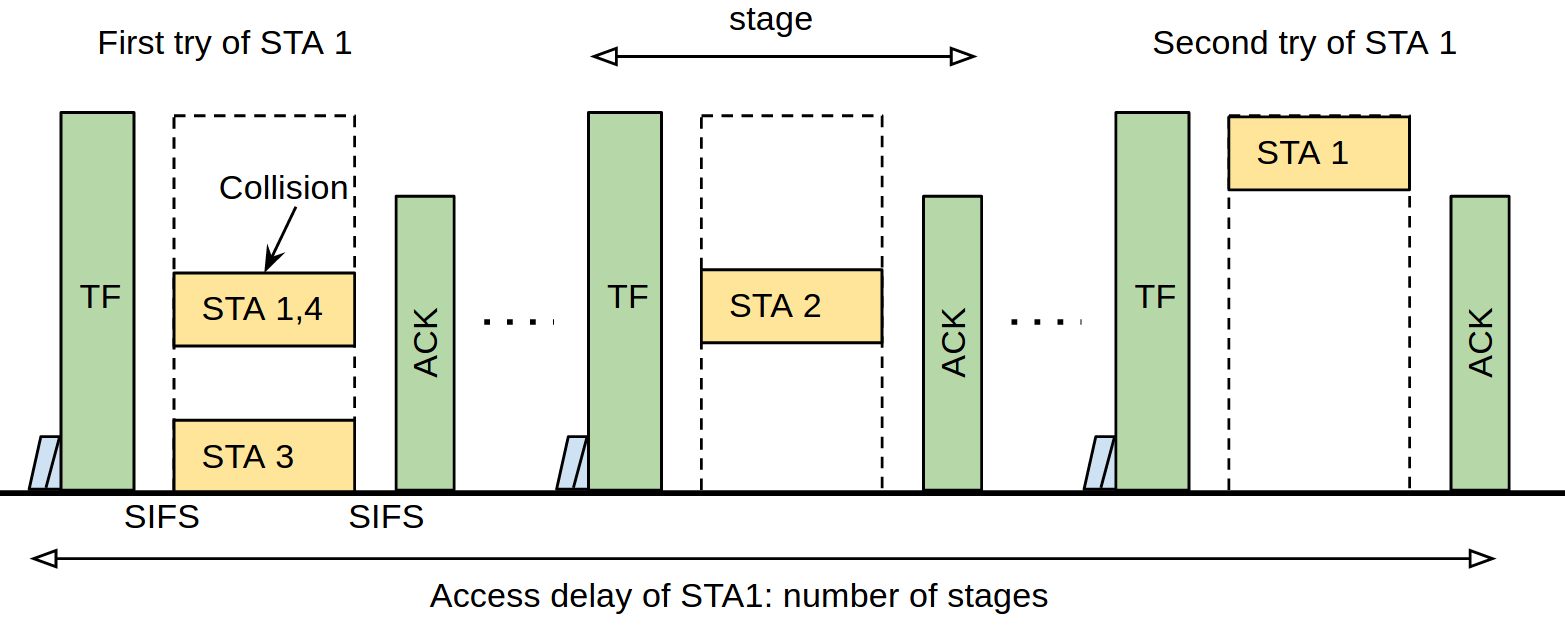
\includegraphics[scale=0.27]{./figure/chp3/ra_time.png}
\caption{Concept of time in OFDMA-based random access}
\label{fig_ra_time}
\end{figure}



\section{Packet Transmission Probability} \label{sec_model}
Since 802.11ax implements OFDMA and trigger-based UL, 802.11ax stations won't contend with AP under this situation.
To estimate the performance of the OFDMA-based random access mechanism, we assume a saturated condition that each station always has requests to transmit.
In the above use case, each station will contend to send \textit{Buffer Status Report} (BSR), for convenience and easy understanding we call it request in the following context, for the data transmission later. 
Consider a fixed number $n$ of contending stations. 
$M$ represents the number of RU for random access in a stage. 


Let $b(t)$ be the stochastic process representing the backoff time counter for a given station.
A discrete and integer time scale is adopted: $t$ and $t+1$ correspond to the beginning of two consecutive stage times, and the backoff time counter of each station decrements at the beginning of each stage.
Note that this discrete time scale does not directly relates to the physical time.
In fact, as illustrated in figure \ref{fig_ra_time}, time interval between two consective stages is variable.
And since the OFDMA-based random access in MU PHY is kind of Aloha random access, the backoff counter will only be frozen outside the stage period. 
The request packet is contained in a stage, thus the time interval between two stages is just a stage, which is absolutely different with Bianchi's model.
In Bianchi's model of DCF, the time interval between two slot time beginnings may be much longer than the slot time size, as it may include a packet transmission. 
That's why in section \ref{sec_metric}, we could generate easy system efficiency rather than a complicate throughput as in \cite{bianchi2000performance}.

Since the value of the backoff counter of each station depends also on its transmission history (e.g., how many retransmission the head-of-line packet has suffered), the stochastic process $b(t)$ is non-Markovian.
However, define convenience $W_0=OCW_{min}$. 
Let $m$, "maximum backoff level", be the value such that $OCW_{max}=2^mW_0$, and let's adopt the notation $W_i$, the OFDMA contention window (OCW) at $i^{th}$ backoff level, with relationship $W_i = 2W_{i-1}+1$, where $i\in (0,m)$ is called "backoff level".
Let $s(t)$ be the stochastic process representing the backoff level $(0,...,m)$ of the station at time $t$.

The key approximation in our model is that, at each transmission attempt, and regardless of the number of retransmissions suffered, each packet collides with constant and independent probability $p$. It is intuitive that this assumption results more accurate as long as $W_0$ and $n$ get larger. $p$ will be referred to as "conditional collision probility", meaning that this is the probability of a collision seen by a packet being transmitted on the channel.

Once independence is assumed, and $p$ is supposed to be a constant value, the bidimensional process $\lbrace s(t),b(t) \rbrace$ could be modeled with Markov chain as in figure\ref{Markov}. 
There mainly two differences compared with Bianchi's Markov chain.
Firstly, since states $( i,0\sim M )$ all means station could access RU, we could merge these states into one state, denoted by $( i, T )$. 
Secondly, at beginning of each stage, the backoff counter will decrease the value of $M$, instead of $1$, which is depicted in chapter \ref{chp_ax_feature}.
\begin{table}[!b]
\caption{Parameters and Notations}
\centering
\label{table_notation}
\begin{tabular}{c|l}
\hline
$n$						& $\#$ of stations \\
$OCW_{min}$ or $W_0$		& minimum OFDMA contention window \\
$M$						& $\#$ of RUs for random access \\
$m$						& maximum backoff level \\
$p$						& packet collision probability \\
$\tau$					& station's transmission probability \\
$n_s$					& $\#$ of successful stations in a stage \\
$D$			            & access delay, $\#$ of stages for a station \\ & to succeed in contending \\
$D_s$					& $\#$ of stages until a successful stage \\
\hline
\end{tabular}
\end{table}

\begin{figure}[!t]
    \centering
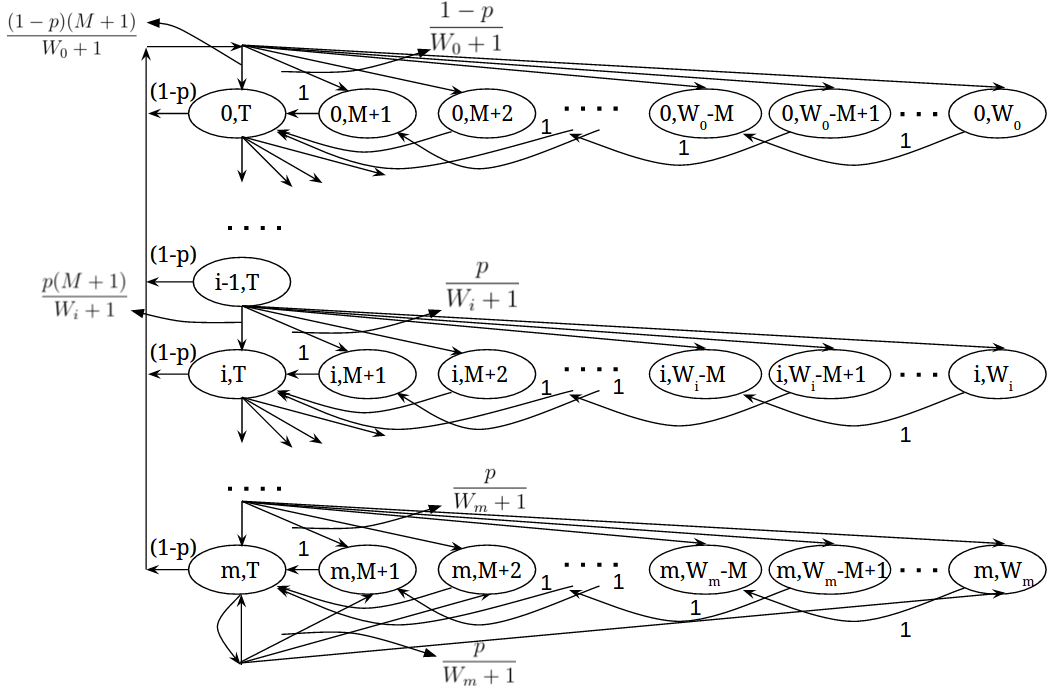
\includegraphics[scale=.4]{./figure/chp3/Markov_chain.png}
\caption{Markov Chain model for the backoff window size}
\label{Markov}
\end{figure}

Let's assume $P\lbrace i_1, k_1|i_0,k_0\rbrace = P\lbrace s(t+1) = i_1, b(t+1)= k_1|s(t) = i_0, b(t) = k_0\rbrace $. In this Markov Chain, the only non null one-step transition probabilities are 
\begin{align}
\left\lbrace
\begin{array}{lll}
P\lbrace i, T | i, k \rbrace = 1  						& k\in [M+1,2M]			& i \in [0,m]\\ [3pt]
P\lbrace i, k-M | i, k \rbrace = 1  						& k\in [2M+1,W_i]   		& i \in [0,m]\\ [3pt]
P\lbrace 0, k | i, T \rbrace = \frac{1-p}{W_0+1}  		& k\in [M+1,W_0]			& i \in [0,m]\\ [3pt]
P\lbrace 0, T | i, T \rbrace = \frac{(1-p)(M+1)}{W_0+1}  &						& i \in [0,m]\\ [3pt]
P\lbrace i, k | i-1, T \rbrace = \frac{p}{W_i+1} 		& k\in [M+1,W_i] 		& i \in [1,m]\\ [3pt]
P\lbrace i, T | i-1, T \rbrace = \frac{p(M+1)}{W_i+1}    &  						& i \in [1,m]\\ [3pt]
P\lbrace m, k | m, T \rbrace = \frac{p}{W_m+1} 		 	& k\in [M+1,W_m] 		& \\ [3pt]
P\lbrace m, k | m, T \rbrace = \frac{p(M+1)}{W_m+1}
\end{array}
\right.
\label{trans_prob}
\end{align}
The first and second equations in \ref{trans_prob} accounts for the fact that in a trigger frame stage for random access, the backoff counter maintained by stations will decrease the number of RUs for random access. 
The third and fourth equation represents that after a successful contention, stations will reset the contention window size to initial window size and uniformly generate a backoff value among $[0,W_0]$, since $T = [0,M]$, the transition probability to $( i, T )$ is $M+1$ times of that to $( i, k )$. 
For the fifth and sixth equations, they represents when a failure contention occurs, the contention window size will be doubled. 
The last two equation is situation of failure contention at the maximum backoff level.

Let $b_{i,k} = \lim_{t\rightarrow \infty} P\lbrace s(t) = i, b(t) = k\rbrace,\ i\in [0,m], \ k \in [0,W_i]$ be the stationary distribution of the Markov chain. Then we show the steady state for the Markov Chain.
First,  for $k = T$
\begin{align}
b_{i-1,T}\cdot p = b_{i,T} 		\rightarrow b_{i,T} = p^i b_{0,T}, \quad 0\leq i < m\\
b_{m-1,T}\cdot p = (1-p) b_{m,T}	\rightarrow b_{m,T} = \frac{p^m}{1-p}b_{0,T}.
\label{biT}
\end{align}

Then, owing to the chain regularities, for each $k\in [T, W_i]$, it is 
\begin{align}
&b_{i,k} = 
\begin{cases}
(\lfloor \frac{W_0-k}{M} \rfloor+1)\frac{(1-p)}{W_0+1}\sum_{i=0}^m b_{i,T}, \  &M+1\leq k\leq W_0,\ i = 0\\[3pt] \nonumber
(\lfloor \frac{W_i-k}{M} \rfloor+1)\frac{p}{W_i+1}b_{i-1,T}, 				\	& M+1 \leq k\leq W_i, \ 0<i<m \\[3pt]
(\lfloor \frac{W_m-k}{M} \rfloor+1)\frac{p}{W_m+1} (b_{m-1,T}+b_{m,T}),  & M+1 \leq k\leq W_m, \ i = m \nonumber 	
\end{cases}
\\
\label{steady_prob}
\end{align}

From equation \ref{biT}, we have $\sum_{i=0}^m b_{i,T}= \frac{b_{0,T}}{1-p}$; sum the equation \ref{steady_prob} respectively which means the sum of each row of states in figure \ref{Markov}, we obtain equation \ref{part_sum}.  

\begin{align}
\begin{cases}
\sum_{k=M+1}^{W_0} b_{0,k} = \frac{b_{0,T}}{W_0+1}\left(-\frac{M}{2}\left\lfloor \frac{W_0}{M}\right\rfloor ^2 + \left(W_0-\frac{M}{2}\right)\left\lfloor \frac{W_0}{M} \right\rfloor \right) \\[3pt]
\sum_{i=1}^{m-1}\sum_{k=M+1}^{W_i} b_{i,k} = \frac{b_{0,T}}{W_0+1}\left(\frac{p}{2}\right)^i \left(-\frac{M}{2}\left\lfloor \frac{W_i}{M}\right\rfloor ^2 + \left(W_i-\frac{M}{2}\right)\left\lfloor \frac{W_i}{M} \right\rfloor \right) \\[3pt]
\sum_{k=M+1}^{W_m} b_{m,k} = \frac{b_{0,T}}{W_0+1}\frac{(\frac{p}{2})^m}{1-p}\left(-\frac{M}{2}\left\lfloor \frac{W_m}{M}\right\rfloor ^2 + \left(W_m-\frac{M}{2}\right)\left\lfloor \frac{W_m}{M} \right\rfloor \right) 
\end{cases}
\label{part_sum}
\end{align}

For convenience, let $X_i = -\frac{M}{2}\left\lfloor \frac{W_i}{M}\right\rfloor ^2 + \left(W_i-\frac{M}{2}\right)\left\lfloor \frac{W_i}{M} \right\rfloor$. Then we are capable of summing all the states to have equation \ref{total_sum2}.
\begin{align}
1 &= \sum_{i=0}^m \sum_{k=0}^{W_i}b_{i,k} 
 = \frac{b_{0,T}}{W_0+1}\left( X_0 + \sum_{i=1}^{m-1}X_i\left( \frac{p}{2}\right)^i + X_m\frac{\left( \frac{p}{2}\right)^m}{1-p}\right) + \frac{b_{0,T}}{1-p}\label{total_sum}\\
& = b_{0,T}\left( \frac{(1-p)X_0+(1-p) \sum_{i=1}^{m-1}X_i\left( \frac{p}{2}\right)^i+X_m\left( \frac{p}{2}\right)^m+W_0+1}{(W_0+1)(1-p)}\right)\label{total_sum2}
\end{align}

We can now express $\tau$, the probability of a station transmit a request at a randomly selected stage.
As any transmission occurs when the backoff time counter is equal to zero, regardless of the backoff level, it is

\begin{align}
\label{tau_general}
\tau &= \sum_{i=0}^m b_{i,T} = \frac{b_{0,T}}{1-p}  \nonumber \\
 &=\frac{W_0+1}{W_0+1+(1-p)X_0+(1-p) \sum_{i=1}^{m-1}X_i\left( \frac{p}{2}\right)^i+X_m\left( \frac{p}{2}\right)^m}
\end{align}

As a side note, it is interesting to highlight that, when $m=0$ (i.e., no exponential backoff is considered), check equation \ref{total_sum}, the terms containing $X_i, i>0$ will disappear, and $b_{0,T}/(1-p)$ will just be $b_{0,T}$.
Thus, equation \ref{total_sum2} will be degraded to 
\begin{align}
1 = b_{0,T}\left( \frac{W_0+1+X_0}{W_0+1}\right),
\end{align}
further simplified that $M=1$ and $X_0=\frac{W_0^2-W_0}{2}$, then
\begin{align}
\tau = b_{0,T} &= \frac{W_0+1}{W_0+1+X_0} \nonumber\\
			   &= \frac{2(W_0+1)}{W_0^2+W_0+2},
\label{tau_W0}
\end{align}
which is different from \cite{ho1996performance} since the OFDMA-based random access is Aloha-like not CSMA-like random access. 
Whatever, the probability $\tau$ results to be independent of $p$.

On the other hand, in general, $\tau$ depends on the conditional collision probability $p$, which is still unknown. To find the value of $p$ it is sufficient to note that the probability $p$ that a transmitted packet encounters a collisions, is the probability that, in a stage, at least one of the $n-1$ remaining stations transmit on the selected RU. 
The fundamental independence assumption given above implies that each transmission "sees" the system in the same state, i.e., the steady state. 
At steady state, each remaining station transmits a packet with probability $\tau$. This yields 
\begin{align}
\label{p_ax}
p = 1-\left( 1-\frac{\tau}{M} \right)^{n-1}.
\end{align}
Rewrite the equation \ref{p_ax}, $\tau^\star = \left(1-(1-p)^\frac{1}{n-1} \right)M$. 
To obtain transmission probability $\tau$ and conditional probability $p$, we need to find solutions to group of equations \ref{tau_general} and \ref{p_ax}.
$\tau^\star(p)$ is a monotonically increasing function. 
Though $\tau(p)$ is hard to determine the monotonicity from the expression of equation \ref{tau_general} with respect to $p$. 
We justify the monotonic decrease of function \ref{tau_general} with numerical method. 
Also, $\tau(0) = \frac{W_0+1}{W_0+1+X_0}> \tau^\star(0) = 0$.
And $\tau(1) < \tau^\star(1) = M$. We find the only solution with numerical method.



\section{Random Access Efficiency} \label{sec_metric}
With the transmit probability, we could easily estimate efficiency of random access mechanism. 
Firstly, find expected number of stations who succeed in contending to transmit request at a stage, which is denoted with $E[n_s]$. 
Extending $n_s$, we define a system efficiency as an important metric.
Secondly, we are interested in the access delay of request frame. 
In another word, say how many stages needed for a station to succeed in contending, denoted by $D$.
What's more, another interesting metric is how many stages are elapsed until a successful stage, which means at least one station succeed in contending in the stage. This metric is a concept similar to "delay" in the second use case of OFDMA-based random access. We represent it with $D_s$. It helps design whole MU UL transmission procedure. 
Here, our concern is mainly on $n_s$, system efficiency and access delay all of which are purely related to random access procedure. The other metric $D_s$ is only expressed in the subsection of access delay, not being discussed later. 

\subsection{$n_s$ and System Efficiency}
What we care in the random access is that how many stations contend successfully in a single stage, denoted by $n_s$.
Given transmission probability $\tau$ and conditional collision probability $p$, we could obtain probability that a station succeeds in contending in a stage, $P_{s\_station} = \tau (1-p)$.
Then, with equation \ref{p_ax}, $E[n_s]$ is easily computed as follows. 
\begin{align}
\label{equ_ns}
E[n_s] &= n P_{s\_station} \nonumber \\
		&= n\tau (1-p) \nonumber \\
		&= n\tau (1-\frac{\tau}{M})^{n-1}
\end{align}

Furthermore, normalizing $n_s$ so that we could compare among different $M$, thus system efficiency is defined as 
\begin{align}
\label{eff_def}
\textit{eff}\ (\tau) &= \frac{E[\text{number of successful stations in a given stage}]}{\text{number of RUs for random access in a stgae}} \nonumber\\
					 &=\frac{E[n_s]}{M} \nonumber \\
					 &= \frac{n\tau(1-\frac{\tau}{M})^{n-1}}{M}.
\end{align}

Both two metrics are our concerns. Another metric, access delay, is derived in next subsection.
With all these metrics, we could evaluate the performance later.

	
\subsection{Access Delay}
Access delay $D$ is defined as number of stages needed for a station to succeed in contending.  
This access delay is different from legacy access delay since the concept of time here is not corresponding with phsical time.
We measure the time as number of stages.
Access delay $D$ follows geometric distribution with parameter $P_{s\_station}$, which is obtained just now.
Thus the expected value of access delay of request frame, $E[D]$, is 
\begin{align}
\label{equ_delay}
E[D] = \frac{1}{P_{s\_{station}}} = \frac{1}{\tau (1-\frac{\tau}{M})^{n-1}}.
\end{align}

Then another interesting metric which is not our focus, denoted by $D_s$, that how many stages are elapsed until a successful stage. 
We could firstly obtain $P_{s\_stage}$, the probability of a successful stage, which means at least one station succeed in contending in the stage.

\begin{align}
P_{s\_stage} &= 1-P\lbrace n_s = 0\rbrace \nonumber \\
	&= 1-(1-P_{s\_station})^n \nonumber\\
	&= 1-(1-\tau(1-p))^n
\end{align} 	 
Since $D_s$ follows geometric distribution with parameter $P_{s\_stage}$,  
\begin{align}
E[D_s] &= \frac{1}{P_{s\_stage}}  \nonumber \\
			&= \frac{1}{1-(1-\tau(1-p))^n}
\end{align} 

In a word, we focus on three metrics: number of successful stations in a stage by $n_s$, system efficiency by $E[n_s]/M$ and access delay given by $D$. 
Actually, only two variables are concerned, $n_s$ and $D$. However, $n_s$ and its normalized value are both meaningful, which we will explain in following sections.


\section{Model Validation} 		\label{sec_model_val}
To validate the Markov chain model, we run a simulation using C language according to the settings as in section \ref{sec_RA_illu}. 
We run the simulation with variety of parameter sets $\lbrace M, OCW_{min}, OCW_{max}\rbrace$ and collects the information of the two variables, $n_s$ and $D$. 
The values of results from both analysis and simulation are given in figure \ref{validation} and table \ref{table_val}. 
All simulation results are obtained from a long-run simulation.
The results show that the Markov model precisely predict the steady state behavior of the OFDMA-based random access.
\begin{table}[!h]
\caption{Analysis versus simulation: $n_s$ and access delay with $m=3,M=9,OCW_{min} = 15$}
\label{table_val}
\begin{center}
\begin{tabular}{c|c|c}
\hline
$n_s$ 	& analysis 	& simulation \\
\hline
$n=1$ 	& 0.72727  	& 0.72728 \\
$n=5$ 	& 2.23001	& 2.22335 \\
$n=10$	& 2.88954	& 2.88546 \\
$n=20$	& 3.29798	& 3.29857 \\
\hline
delay	& analysis	& simulation \\
\hline
$n=1$ 	& 1.37500  	& 1.37499 \\
$n=5$ 	& 2.24214	& 2.24886 \\
$n=10$	& 3.46075	& 3.46565 \\
$n=20$	& 6.06432	& 6.06323 \\
\hline
\end{tabular}
\end{center}
\end{table}

\begin{figure}[!h]
    \centering
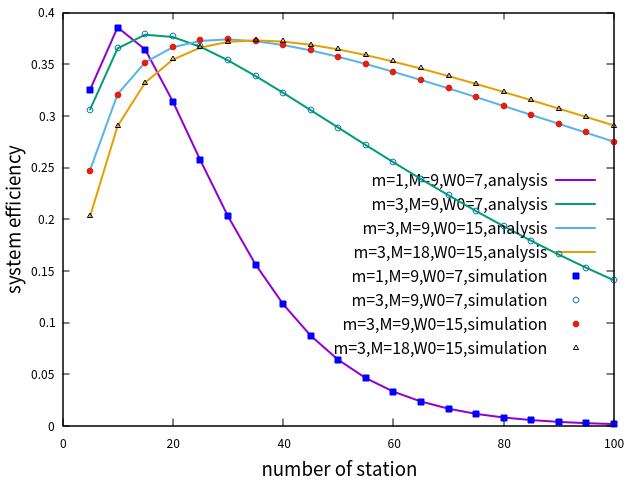
\includegraphics[scale=0.74]{./figure/chp3/multiple_parameter.png}
\caption{System efficiency: Analysis versus Simulation}
\label{validation}
\end{figure}
